\documentclass{article}
\usepackage[utf8]{inputenc}
\usepackage{algorithm}
\usepackage{algpseudocode}
\usepackage{graphicx}
\usepackage{amsmath,amssymb,amsthm, ,amsfonts}

\title{Location Prediction Algorithm}
\author{Shashank Sharma }
\date{August 2018}

\begin{document}

\maketitle

\section{Introduction}
This algorithm is designed to predict human locations in a real world scenario. The GPS data is taken as input and the processed using the below algorithm.


The Algorithm has several steps:
\begin{itemize}
\item Detect stay-points (also detect start or end of the trajectory)
\item Group stay-points to form states
\item Calculate hourly weights for the states
\item Apply Markov chain for the data available
\end{itemize}

\begin{figure}[h!]
\centering
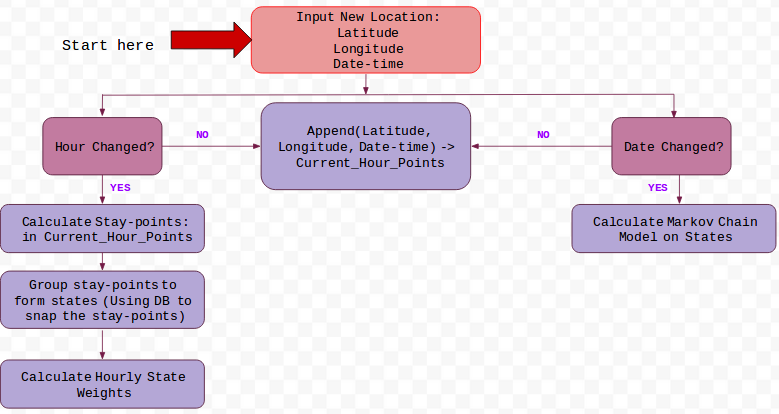
\includegraphics[scale=.46]{Flowchart_Algo.png}
\caption{Algorithm Flow-chart}
\label{fig:flow-chart}
\end{figure}

\begin{figure}[h!]
\centering
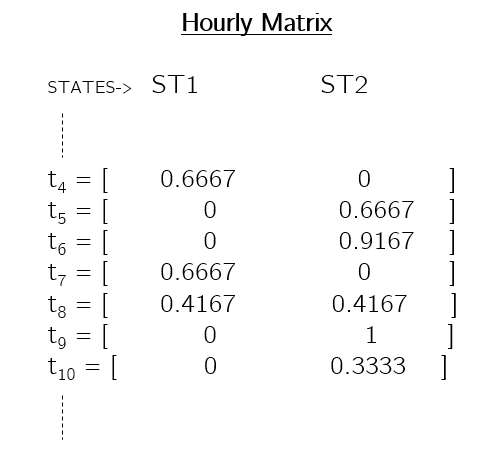
\includegraphics[scale=.34]{hourlymat.png}
\caption{Algorithm Flow-chart}
\label{fig:flow-chart}
\end{figure}

\begin{figure}[h!]
\centering
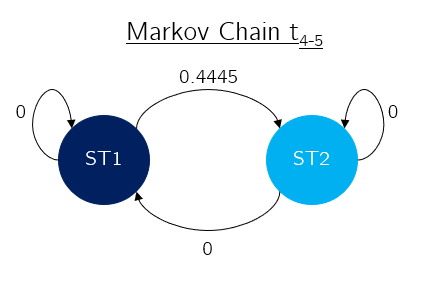
\includegraphics[scale=.35]{markovchain.png}
\caption{Algorithm Flow-chart}
\label{fig:flow-chart}
\end{figure}

\begin{figure}[h!]
\centering
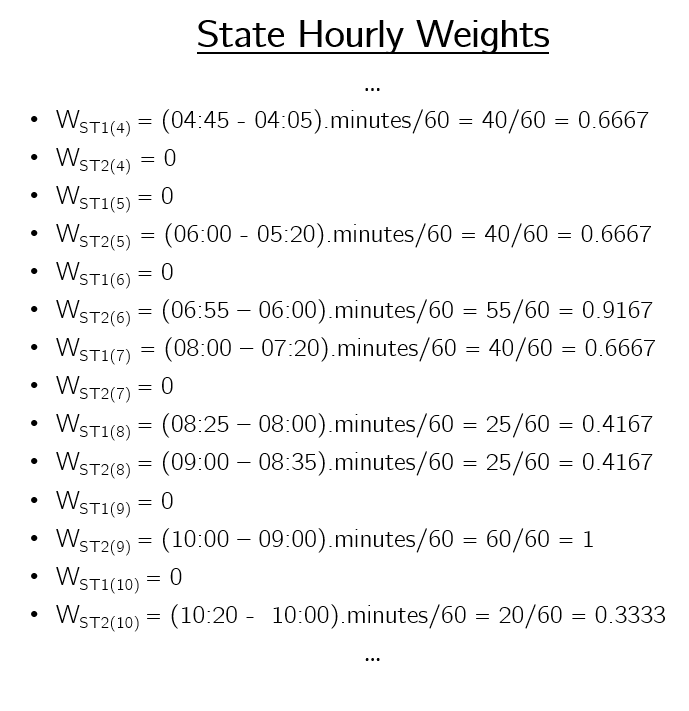
\includegraphics[scale=.35]{stateweights.png}
\caption{Algorithm Flow-chart}
\label{fig:flow-chart}
\end{figure}

\begin{figure}[h!]
\centering
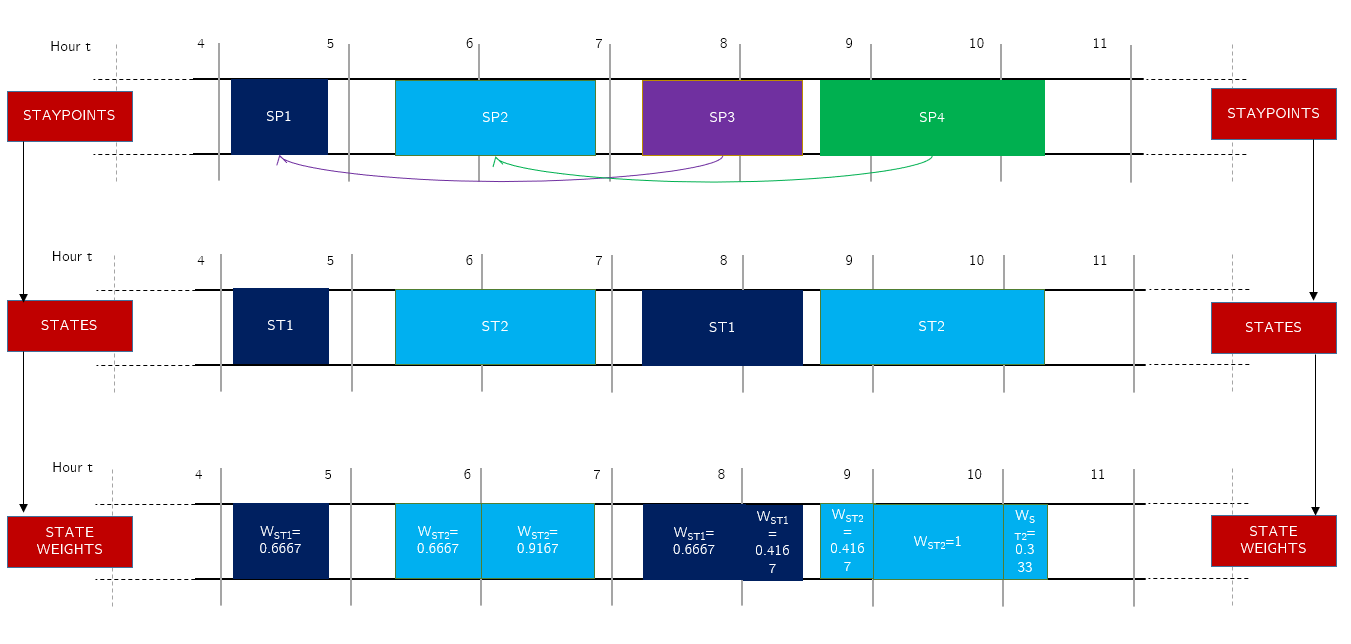
\includegraphics[scale=.54]{threestepsover.png}
\caption{Algorithm Flow-chart}
\label{fig:flow-chart}
\end{figure}

\section{Definitions}
\begin{itemize}
	\item \textbf{Stay-points:} Stay-points are any points which are stayed by the user in user trajectories or it is the start or the end of the trajectory. For example, if user start at his home, the home itself is a stay-point. Now he move towards work, but he visit a cafe in between for breakfast. The cafe is also a stay-point and then he finishes his trajectory at work, where work is again a stay-point. The places like cafe in this case is identified using distance and time based clustering. For example, a set of points within 200m with total duration of stay greater than 20 minutes can be regarded as a stay-point within the trajectory.
	\item \textbf{State:} A state is formed using a group of stay-points. This is done using a distance threshold for states. All the stay-points within this threshold distance are grouped together as a single state. This is called snapping stay-points to the states. The mean of all location latitudes and longitudes from stay-points within a state are stored per state. Finally Markov Chain model is applied to the states. \textit{Note: A new stay-point is only added to the state if after calculating the mean of the new state, all the existing stay-points still stay within the distance threshold from this mean. This is done to avoid drifting problem while aggregating the stay-points into states.}
\end{itemize}

\section{Algorithms}

\iffalse
\begin{algorithm}
\caption{Read new location and process}
\label{pseudoPSO}
\hspace*{\algorithmicindent} \textbf{Input:} \text{GPS Points} \textit{P[x, y, d]} \\
\hspace*{\algorithmicindent} \textbf{Output:} \text{Markov Chain} \textit{mc} 
\begin{algorithmic}[1]
\For{each \textit{P[x, y, d]}}
\State $newHour \gets d_h$
\State $newDate \gets d_d$
\If{$newHour != prevHour$}
	\State $prevHour \gets newHour$
	\State extractStayPoints()
	\State formStates()
	\State calculateStateWeights()
	\If{$newDate != prevDate$}
		\State $prevDate \gets newDate$
		\State updateMarkovModel()
	\EndIf
	\State clear \textit{lst\_hr\_pts[x, y, d]}
\Else
	\State $lst\_hr\_pts[x, y, d] \gets P[x, y, z]$
\EndIf
\EndFor
\end{algorithmic}
\end{algorithm}
\fi

\begin{algorithm}
\caption{extractStayPoints() : Calculate stay-points}
\label{pseudoPSO}
\hspace*{\algorithmicindent} \textbf{Input:} \text{Last hour GPS points} \textit{lst\_hr\_pts[x, y, d]} \\
\hspace*{\algorithmicindent} \textbf{Output:} \text{Stay-points} \textit{sp} 
\begin{algorithmic}[1]

\For{each  \textit{lst\_hr\_pts[x, y, d]\textsubscript{i}} in \textit{lst\_hr\_pts[x, y, d]}}
\If{$d\textsubscript{i} - d\textsubscript{i+1} > th\_tck$}
	\State$ sp \gets lst\_hr\_pts\textsubscript{i},  lst\_hr\_pts\textsubscript{i+1}$
\ElsIf{$distanceBtw( lst\_hr\_pts\textsubscript{i}, cluster) <=   th\_d$}
	\State $cluster \gets lst\_hr\_pts\textsubscript{i}$ 
	\State Update Cluster Mean
\ElsIf{$(cluster != empty$) And $duration(cluster) >= th\_t$}
    \State $sp \gets cluster$
\EndIf

\EndFor
\end{algorithmic}
\end{algorithm}

\begin{algorithm}
\caption{adjustStartEndStaypoint() : Adjust start-end time of stay-points}
\label{pseudoPSO}
\hspace*{\algorithmicindent} \textbf{Input:} \text{Stay-points} \textit{sp} \\
\hspace*{\algorithmicindent} \textbf{Output:} \text{Stay-points with adjusted start and end points} \textit{sp}
\begin{algorithmic}[1]
\For{each \textit{sp\textsubscript{i}} in \textit{sp}}
	\State $d \gets distanceBtw(sp\textsubscript{i}, sp\textsubscript{i+1})$
	\State $t \gets timeDiff(sp\textsubscript{i}, sp\textsubscript{i+1})$
	\State $s \gets d/t$
	\If {$s != 0$}
		\State $delta\_t \gets min(d$, $th\_d)/s$
	\Else
		\State $delta\_t \gets t/2$
	\EndIf
	\State Update end\_time \textit{d\textsubscript{e}+delta\_t/2}  for \textit{sp\textsubscript{i}}
	\State Update start\_time \textit{d\textsubscript{s}-delta\_t/2} for \textit{sp\textsubscript{i+1}}
\EndFor
\end{algorithmic}
\end{algorithm}


\begin{algorithm}
\caption{formStates() : Form states from stay-points}
\label{pseudoPSO}
\hspace*{\algorithmicindent} \textbf{Input:} \text{Stay-point} \textit{sp\textsubscript{n+1}} \text{, States} \textit{st} \\
\hspace*{\algorithmicindent} \textbf{Output:} \text{States} \textit{st}

\begin{algorithmic}[1]

\For{each \textit{st\textsubscript{j}} in \textit{st}}
\State $is\_sp\textsubscript{n+1}\_added \gets False$
\If{$distanceBtw(sp\textsubscript{n+1}, st\textsubscript{j}) <= th\_d$}
	\State Add sp\textsubscript{n+1} to st
	\State $newMean \gets mean(\textit{st})$
	\If {$distanceBtw(All$ $sp's$ $of$ $st\textsubscript{j}, newMean) <= th\_d$}
		\State Add \textit{sp\textsubscript{n+1}} to \textit{st\textsubscript{j}}
		\State $is\_sp\textsubscript{n+1}\_added \gets True$ 
		\State Break
	\Else
		\State Remove sp\textsubscript{n+1} from st
	\EndIf
\EndIf
\EndFor
\If{$is\_sp\textsubscript{n+1}\_added=False$}
\State Add new state in st
\EndIf
\end{algorithmic}
\end{algorithm}

\iffalse
\begin{algorithm}
\caption{calculateStateWeights() : Calculate Hourly Weights of States}
\label{pseudoPSO}
\hspace*{\algorithmicindent} \textbf{Input:} \text{States} \textit{st} \\
\hspace*{\algorithmicindent} \textbf{Output:} \text{States Weights} \textit{w}
\begin{algorithmic}[1]
\State This creates a weights of all states from 0 Hrs to 24 Hrs for each date
\For{each \textit{st\textsubscript{i}} in \textit{st}}
	\State $w\textsubscript{i} \gets minutesContribution(st\textsubscript{i}) / 60$
\EndFor
\end{algorithmic}
\end{algorithm}
\fi

\begin{algorithm}
\caption{markovModel() : Create the Markov Model with transition probabilities)}
\label{pseudoPSO}
\hspace*{\algorithmicindent} \textbf{Input:} \text{State Weights} \textit{w} \\
\hspace*{\algorithmicindent} \textbf{Output:} \text{Markov Chain Model} \textit{mc}
\begin{algorithmic}[1]
\For{each $h-hour$ from $0to23$ }
	\If {$h!=23$}
		\State $trn\_mat\textsubscript{h+1} \gets w\textsuperscript{h\textsuperscript{\text{[T]}}} * w\textsuperscript{h+1}$
		\State $mc\textsubscript{h+1} \gets eachCell(trn\_mat\textsubscript{h+1})/rowSum(trn\_mat\textsubscript{h+1})$
	\Else
		\State $trn\_mat\textsubscript{0} \gets w\textsuperscript{23\textsuperscript{\text{[T]}}} * w\textsuperscript{0}$
		\State $mc\textsubscript{0} \gets eachCell(trn\_mat\textsubscript{0})/rowSum(trn\_mat\textsubscript{0})$
	\EndIf
\EndFor
\end{algorithmic}
\end{algorithm}

\end{document}



